\documentclass[11pt,a4paper]{article}
\usepackage[margin=2.2cm]{geometry}
\usepackage{graphicx}
\usepackage{booktabs}
\usepackage{amsmath,amssymb}
\usepackage{float}
\usepackage{caption}
\usepackage{subcaption}
\usepackage{hyperref}
\usepackage{multirow}
\usepackage{setspace}
\usepackage{natbib}
\usepackage{xcolor}
\setstretch{1.18}
\hypersetup{colorlinks=true,linkcolor=blue,citecolor=blue,urlcolor=blue}

\title{\textbf{Interpretable Molecular Lipophilicity Prediction Using Enhanced Structural Features, Ensemble Learning, Scaffold-Aware Validation, and Platform Deployment}}
\author{Computational Pharmacy Project Team}
\date{March 2026}

\begin{document}
\maketitle
\begin{abstract}
Lipophilicity is a key physicochemical property in drug discovery and strongly influences membrane permeability, distribution, and developability. We present an end-to-end molecular property prediction workflow using a real public lipophilicity dataset containing 4,200 compounds. Molecular representation integrates RDKit descriptors, Morgan fingerprints, and MACCS keys. We compare baseline and enhanced machine learning models and obtain the best random-split performance using a weighted ensemble model ($R^2 = 0.7232$, $RMSE = 0.6346$, $MAE = 0.4517$). To improve scientific rigor, we further conduct repeated scaffold-aware validation, where the best model remains stable ($R^2 = 0.7138 \pm 0.0215$, $RMSE = 0.6489 \pm 0.0296$). SHAP-based explainability identifies chemically meaningful determinants of prediction, including MolLogP and polarity-related feature groups. Finally, we package the workflow into a deployable web platform with API support and optional Gemini-assisted explanation. This project demonstrates how a modern QSAR system can be simultaneously predictive, interpretable, rigorously validated, and deployment-ready.
\end{abstract}

\section{Introduction}
Molecular lipophilicity is central to the balance between permeability and solubility in medicinal chemistry. Reliable prediction of lipophilicity before experimental testing is useful for candidate prioritization and property optimization. However, predictive performance alone is not sufficient in practice: robust validation and interpretability are equally important.

This work aims to develop a realistic and defensible QSAR-like workflow that integrates (i) real public data, (ii) feature-rich molecular representation, (iii) ensemble learning, (iv) scaffold-aware validation, (v) SHAP explainability, and (vi) lightweight platform deployment.

\section{Materials and Methods}
\subsection{Dataset}
We use the public Lipophilicity dataset with 4,200 molecules and experimentally measured values. Molecules were standardized and deduplicated before modeling.

\subsection{Feature Representation}
Three families of molecular information were used:
\begin{itemize}
    \item basic and extended RDKit descriptors,
    \item Morgan fingerprints,
    \item MACCS keys.
\end{itemize}

\subsection{Modeling Strategy}
We first established baseline models and then enhanced models. The final enhanced system included XGBoost, CatBoost, and a PyTorch MLP. Their outputs were combined through validation-optimized weighted ensembling.

\subsection{Evaluation Strategy}
We report standard regression metrics ($R^2$, RMSE, MAE) under two settings:
\begin{enumerate}
    \item stratified random split,
    \item repeated scaffold-aware split.
\end{enumerate}
The second setting was included to better approximate structural extrapolation to unseen scaffolds.

\section{Results}
\subsection{Random-Split Performance}
The best enhanced model was the weighted ensemble.

\begin{table}[H]
\centering
\caption{Random-split test performance.}
\begin{tabular}{lccc}
\toprule
Model & $R^2$ & RMSE & MAE \\
\midrule
Weighted Ensemble (enhanced) & 0.7232 & 0.6346 & 0.4517 \\
XGBoost (enhanced) & 0.7043 & 0.6559 & 0.4810 \\
CatBoost (enhanced) & 0.6973 & 0.6637 & 0.4862 \\
PyTorch MLP (enhanced) & 0.6967 & 0.6643 & 0.4634 \\
XGBoost (baseline) & 0.6835 & 0.6787 & 0.5075 \\
\bottomrule
\end{tabular}
\end{table}

\begin{figure}[H]
    \centering
    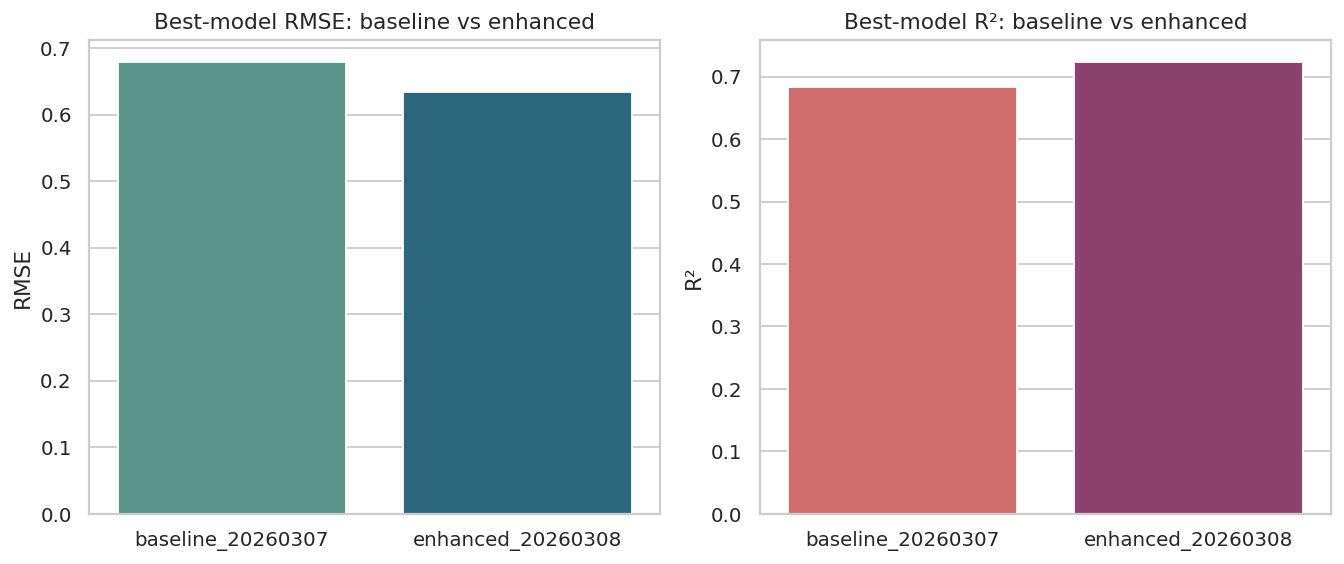
\includegraphics[width=0.85\textwidth]{../figures/14_baseline_vs_enhanced.png}
    \caption{Comparison between baseline and enhanced modeling performance.}
\end{figure}

\subsection{Repeated Scaffold Validation}
To avoid overestimating generalization due to random split similarity, we conducted repeated scaffold-aware validation. The enhanced ensemble remained the best-performing model.

\begin{table}[H]
\centering
\caption{Repeated scaffold-aware validation summary.}
\begin{tabular}{lccc}
\toprule
Model & $R^2$ mean $\pm$ sd & RMSE mean $\pm$ sd & MAE mean $\pm$ sd \\
\midrule
Weighted Ensemble (scaffold) & $0.7138 \pm 0.0215$ & $0.6489 \pm 0.0296$ & $0.4962 \pm 0.0226$ \\
PyTorch MLP (scaffold) & $0.6945 \pm 0.0261$ & $0.6698 \pm 0.0200$ & $0.5111 \pm 0.0187$ \\
XGBoost (scaffold) & $0.6847 \pm 0.0234$ & $0.6811 \pm 0.0347$ & $0.5241 \pm 0.0252$ \\
CatBoost (scaffold) & $0.6750 \pm 0.0234$ & $0.6914 \pm 0.0295$ & $0.5313 \pm 0.0201$ \\
XGBoost baseline (scaffold) & $0.6472 \pm 0.0311$ & $0.7200 \pm 0.0299$ & $0.5519 \pm 0.0234$ \\
\bottomrule
\end{tabular}
\end{table}

\begin{figure}[H]
    \centering
    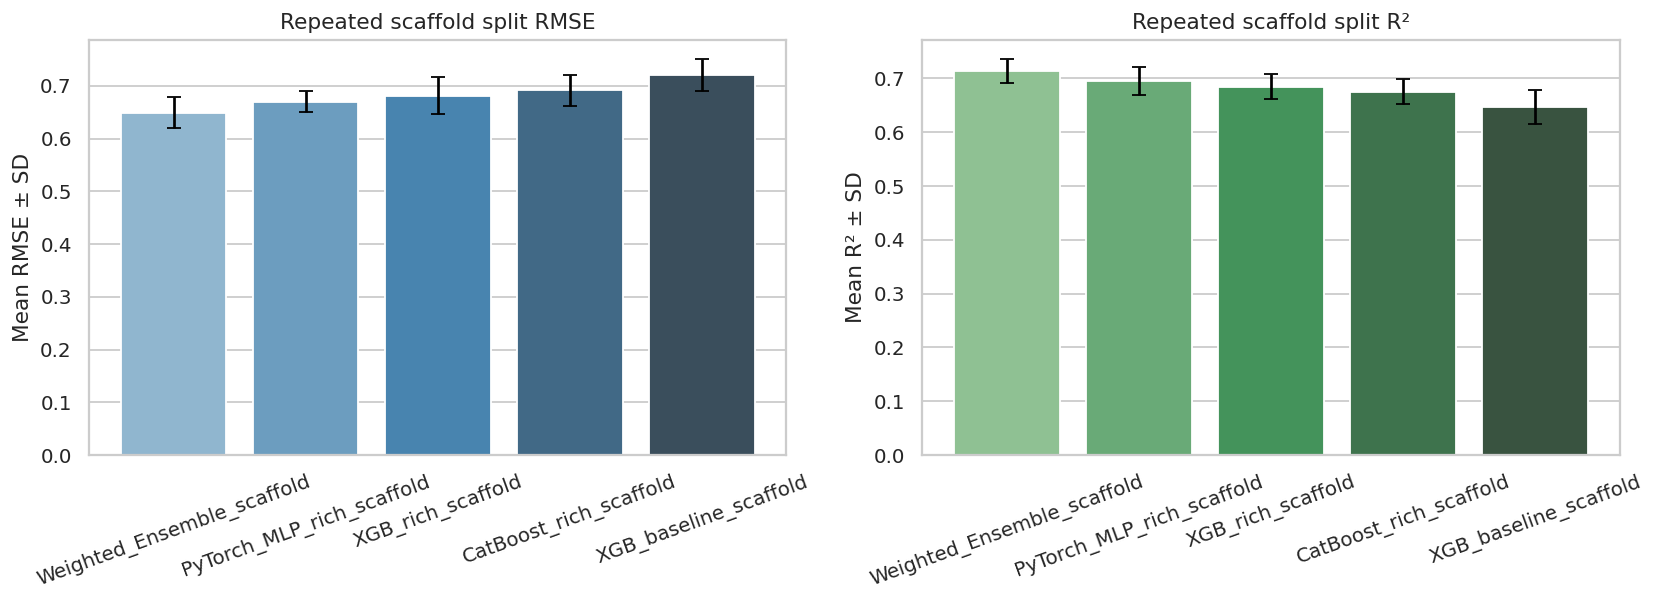
\includegraphics[width=0.88\textwidth]{../figures/16_scaffold_repeat_summary.png}
    \caption{Repeated scaffold-aware validation results.}
\end{figure}

\subsection{Explainability}
Global SHAP analysis highlighted chemically meaningful features. The most influential feature was MolLogP, followed by polarity- and fragment-related indicators such as \texttt{fr\_COO}, \texttt{VSA\_EState5}, and specific MACCS or fingerprint bits.

\begin{figure}[H]
    \centering
    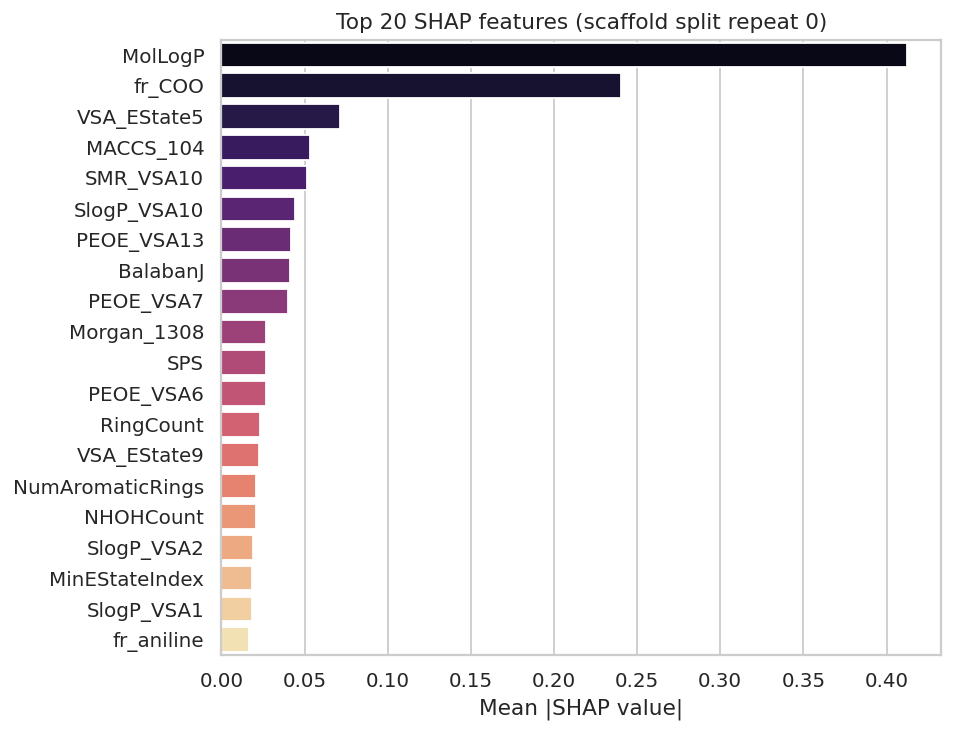
\includegraphics[width=0.78\textwidth]{../figures/19_shap_top20_bar.png}
    \caption{Global SHAP feature importance.}
\end{figure}

Local case analysis further demonstrated how different structural factors could push prediction higher or lower for individual molecules.

\begin{figure}[H]
    \centering
    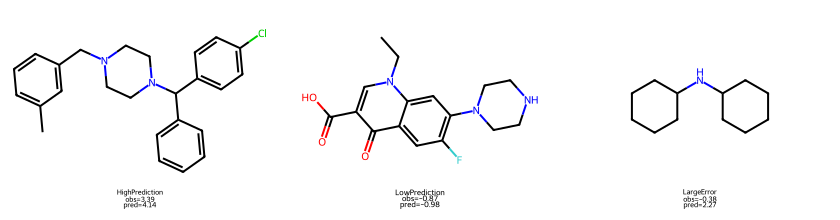
\includegraphics[width=0.78\textwidth]{../figures/22_shap_case_molecules.png}
    \caption{Representative local explanation cases.}
\end{figure}

\section{Discussion}
The project shows that performance gains from richer structure representation are not merely cosmetic. They persist across a stricter scaffold-aware setting, which is especially important for defending model credibility in drug discovery contexts. The SHAP analysis also helps move the system from a pure black-box predictor to a chemically interpretable decision aid.

An additional strength of the project is engineering completeness: the workflow does not stop at model benchmarking, but continues to deployment through a Flask-based Hugging Face Space with API access. The optional Gemini-assisted explanation layer is designed as a language-level interpretation interface rather than a replacement for the predictive model.

\section{Conclusion}
This work presents a complete and defensible lipophilicity prediction workflow that combines enhanced structural features, ensemble learning, repeated scaffold-aware validation, SHAP explainability, and deployment-ready implementation. The resulting system is predictive, interpretable, and suitable for cross-disciplinary presentation in both research and product-style settings.

\end{document}
